\subsection{Stimuli}

\centerline{\textbf{Hur viktigt är stimuli för 
din användarupplevelse}}

\begin{figure}[H]
  \centering
  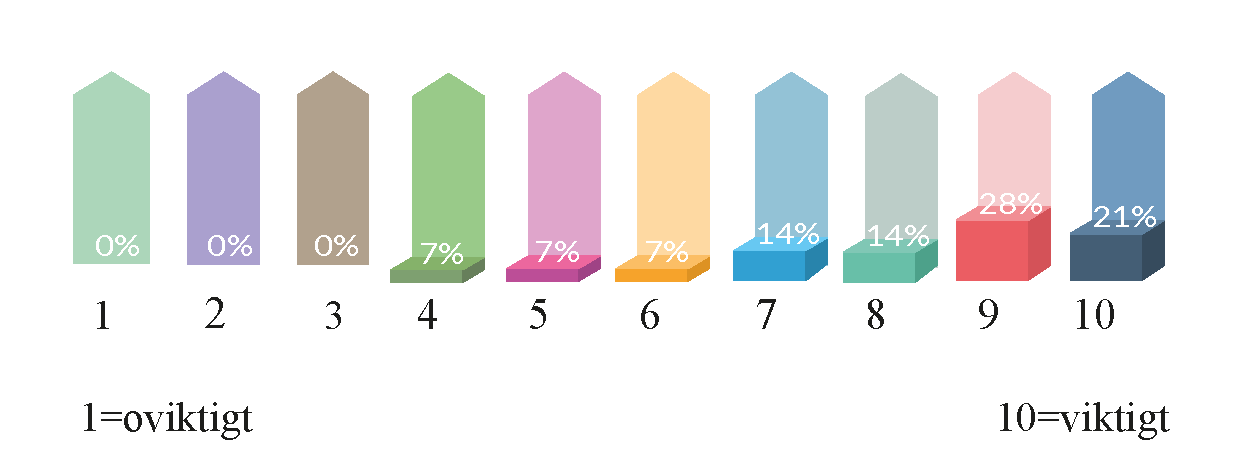
\includegraphics[scale=0.7]{Rityta_12.pdf}
  \centering
  \captionsetup{justification=centering,margin=2cm}
  \caption{Resultat i procentuell skala på respondenternas svar}
\end{figure} 

Medelvärdet av ovan figur är 7.93. Siffran representerar ett medelsnitt av stapeldiagrammet som visar hur viktigt det var för användarupplevelsen enligt kategoriseringen framtagen av Laugwitz et al \cite{Laugwitz2008ConstructionQuestionnaire}. 

%\[
 % m = \frac{4 +5 + 6 + 14 + 16 + 36 + 30}{14} = 7.93
 % \]
  
%Med en standardavvikelse på

%\[
 %\sigma = \sqrt{V} = \sqrt{ \frac{(4-1)^{2} + (5-1)^{2} + (6-1)^{2} + (7-2)^{2} + (8-2)^{2}+ (9-4)^{2} + (10-3)^{2} } {7}} \] 
 %\[
 %= \sqrt{26.43} = 5.14 \]

\newpage
\begin{figure}[H]
  \centering
  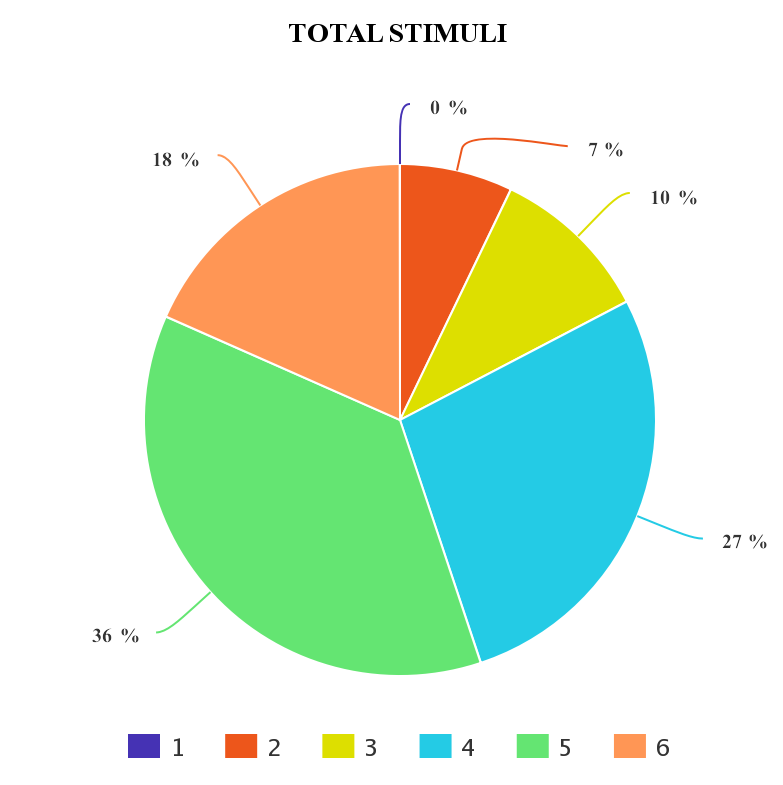
\includegraphics[scale=0.4]{meta-chart-5.png}
  \captionsetup{justification=centering,margin=2cm}
  \caption{Resultat av total stimuli}
\end{figure} 
Figuren visar det slutgiltiga resultatet från både enkätundersökningen samt fokusgrupperna. Figuren visar sambandet mellan hur viktigt stimuli är för användarupplevelsen i en applikation kontra hur stimulerande prototypen känts. Den första rutan visar på hur viktigt det är för användaren att en applikation är stimulerande, enligt personerna som medverkade i fokusgrupperna. Denna siffran beräknades med hjälp av snitt och varians och presenteras nedan. Diagrammen visar på hur stimulerande prototypen kändes, enligt användarna som svarade på enkätundersökningen. 

\textbf{Citat från fokusgrupperna}
%\begin{quotation}
%\em %vad har hänt innan appen? Vi säger om allt annat har fungerat så är appen inte viktig, jag skulle lägga mer krut på vad som är utanför appen snarare än vad som är inuti. 
%\end{quotation}

\begin{quotation}
\em  Utifrån hur Amazing Leaders jobbar här och nu så tror jag att det kan vara ett bra stöd, som en brygga in och för att få kontinuitet
\end{quotation}

\begin{quotation}
\em  Jag gillade interaktivitet i den, och att det var interaktivitet som var personlig för mig. Det tror jag är nyckeln, att det inte är generellt för alla, göra något och reflektera är viktigt. 
\end{quotation}

\begin{quotation}
\em Skulle nog vilja att det fanns en fördjupningsknapp om man ex skulle vilja läsa mer om vad EQ var, vad menas med vad som var mina actions. Då får man ännu en nivå på det 
\end{quotation}

%\begin{quotation}
%\em %Om vi har haft ett möte med, säg Ursula nu då, så har vi dessa tre aktiviteter och övningar som vi har på papper och som vi kan följa upp.
%\end{quotation}

%\begin{quotation}
%\em  %Den andra biten som jag tror kan va intressant också är den här resultat effekten, nån action därefter. vi säger det här kontraktet du har gjort i nån form utav fysiks dialog, dokumentationen och exekveringen utav det långsiktiga är något man kan bocka av.
%\end{quotation}


%\begin{quotation}
%\em %The app should support growth so it does not have to be fun, maybe it should not be fun, then it won’t be serious. It should tot boring but not like a game either. 
%\end{quotation}
